\documentclass{article}
\usepackage{graphicx}
\usepackage[margin=1.5cm]{geometry}
\usepackage{amsmath}

\begin{document}
\twocolumn

\title{Wednesday warm-up: Forces III and Forces IV}
\author{Prof. Jordan C. Hanson}

\maketitle

\section{Memory Bank}

\begin{itemize}
\item Force of drag, in air or other gas: $F_D = \frac{1}{2}C \rho A v^2$.
\item In the above formula, $C$ is an empirical constant, $\rho$ is the density of the air or gas, $A$ is the area of the object, and $v$ is the object's velocity.
\item Spring force: $\vec{s} = -k \Delta \vec{x}$, where $k$ is the spring constant and $\Delta\vec{x}$ is the displacement.
\item The horizontal force of friction: $\vec{f} = -\mu N \hat{i}$, where $\mu$ can be either the \textit{static} or \textit{kinetic} coefficient of friction.
\item \textit{Young's Modulus} relates \textit{stress} to \textit{strain} in a mechanical system.
\item Young's Modulus, $Y$, has units of N m$^{-2}$, and it relates the change in length $\Delta L$ of a system of original length $L_0$ and cross-sectional area $A$ subject to a force $F$:
\begin{equation}
\frac{\Delta L}{L_0} = \frac{1}{Y} \frac{F}{A}
\end{equation}
\end{itemize}

\section{Springs and Restoring Forces}

\begin{enumerate}
\item Consider Fig. \ref{fig:1}.  (a) Derive an expression for the displacement of the spring from its unstretched length, given $m$, $\theta$, and $k$. (b) Assume $m = 1.0$ kg, $\theta = 45$ degrees, and $k = 1$ N m$^{-1}$.  What is $\Delta x$, the displacement of the spring? \\ \vspace{2.5cm}
\item Consider Fig. \ref{fig:2}. (a) The ``lead'' in pencils is a graphite composition with a Young’s modulus of about $10^9$ N m$^{-2}$. Calculate the change in length of the lead in an automatic pencil if you tap it straight into the pencil with a force of 4.0 N. The lead is 0.50 mm in diameter and 60 mm long. (b) Is the answer reasonable? That is, does it seem to be consistent with what you have observed when using pencils?  \\ \vspace{2.5cm}
\end{enumerate}

\begin{figure}[hb]
\centering
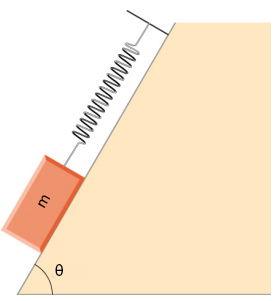
\includegraphics[width=0.25\textwidth]{figures/spring_incline.png}
\caption{\label{fig:1} A spring with spring constant $k$ supports a mass $m$ on an incline with angle $\theta$.}
\end{figure}

\begin{figure}[hb]
\centering
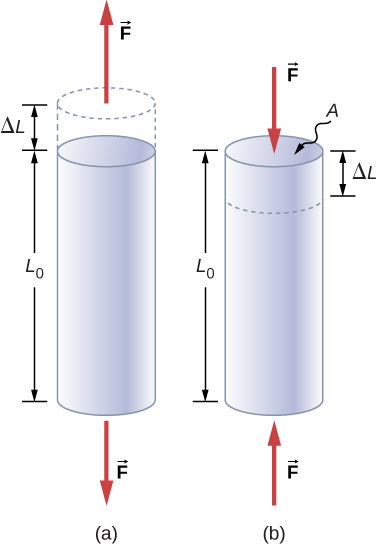
\includegraphics[width=0.25\textwidth]{figures/strain.jpeg}
\caption{\label{fig:2} A spring with spring constant $k$ supports a mass $m$ on an incline with angle $\theta$.}
\end{figure}


\end{document}
